
%%% Local Variables:
%%% mode: latex
%%% TeX-master: "chapter01"
%%% End:

\chapter{数据查询系统更新}
数据查询系统在深圳市交通仿真系统( 二期) 的体系中属于直接面向用户的
GIS 可视化系统, 因此除了后台数据库的更新之外, 还需要对前端的界面功能也
做相应的更新,使用户能够在浏览器界面中查询到 2017 年更新后的指标成果。
所以, 数据查询系统的年度更新主要包括后台数据库的更新和前端功能更新两部分工作。

\section{后台数据库更新}
上节数据挖掘的成果经过汇总运算后,已经推送至数据查询系统后台的指标
数据库, 但是一方面推送的数据中只包含以关系数据表形式存储的指标数据, 并
没有 GIS 图形数据; 另一方面,涉及到路段车速、 OD 流量等大数据量的查询,
为了提高查询效率,深圳市交通仿真系统( 二期) 采用物化视图技术对这些指标
成果进行物理存储,因此需要对这部分物化视图进行更新。

\subsection{GIS 图层数据更新} \label{subsec:GIS 图层数据更新}
GIS 图层数据的更新工作是在第二节数据更新的基础上开展的。 经过第二节
的数据更新工作之后, 编辑完成的静态 GIS 数据以 shapefile 的形式保存在本地
机器上, GIS 图层数据更新工作就是将这些更新后的 shapefile 图层文件导入到数
据查询系统后台的空间数据库中,替换原有图层, 使得在查询系统前端能够展现
最新的 GIS 图层数据。 具体操作步骤如下:

\begin{nbeae}
\item 打开ArcCatalog,在左侧Catalog Tree窗体中找到并展开Database
Connections 节点,找到查询系统后台空间数据库连接“connection to
192.168.114.111.sde” , 并且双击后展开该连接(见图\ref{fig:chp07_打开空间数据库连接});

\begin{figure}[!ht]
  \centering
  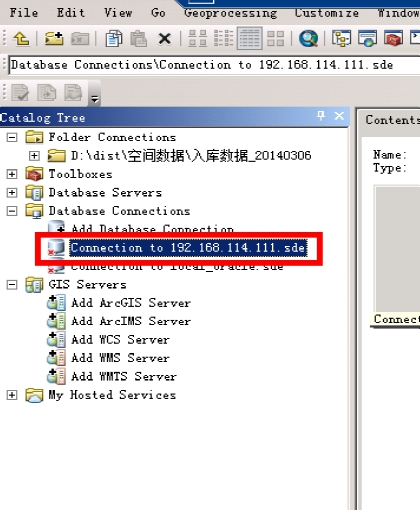
\includegraphics[width=0.5\textwidth]{chp07_打开空间数据库连接.jpg}
  \caption{打开空间数据库连接\label{fig:chp07_打开空间数据库连接} }
\end{figure}

\item 在列表中找到 GIS\_T 开头的 GIS 图层数据,在右击原有的 BusLink,BusRoute,
BusStop, RoadLink 和 RoadNode 图层节点,在弹出的列表中选择 rename 功
能, 将原有图层名分别重命名为 BusLink\pyear, BusRoute\pyear, BusStop\pyear,
RoadLink\pyear 和 RoadNode\pyear;

\item 返回 connection to 192.168.114.111.sde 连接节点,右键打开功能列表,选择
import$\rightarrow$Feature Class (multiple)功能, 打开 Feature Class to Feature Class 对话
框,在 Input Features 中输入\ref{sec:静态GIS数据处理}节更新后的静态 GIS 图层数据,Output Feature
Class 中输入重命名前对应的图层名, 例如公交站点输入 BusStop;

\begin{figure}[!ht]
  \centering
  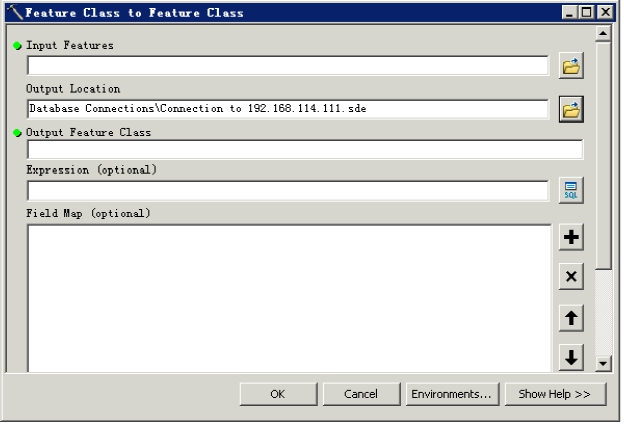
\includegraphics[width=0.8\textwidth]{chp07_向空间数据库中导入数据.jpg}
  \caption{向空间数据库中导入数据\label{fig:chp07_向空间数据库中导入数据} }
\end{figure}

\item 最后,点击 OK 按钮将更新后的\pyear 年GIS图层数据导入查询系统后台空间数据库中。
\end{nbeae}

\subsection{物化视图更新}
物化视图的更新工作需要在所有数据挖掘工作完成后才能进行, 是在数
据库表更新的基础上,通过 Oracle 视图刷新功能将深圳市交通仿真系统( 二期)
中设计的查询系统后台物化视图进行重新运算。由于数据量较大, 这部分工作所
花费的时间会比较长。

深圳市交通仿真系统( 二期) 中设计的物化视图在数据库后台都是在 szyw
表空间下以“ MV\_” 开头存储的,需要更新的全部物化视图列表如下:

\renewcommand{\arraystretch}{0.8}
\begin{longtable}[c] {|C{0.35\textwidth}|C{0.35\textwidth}|}
  \caption{需要更新的物化视图列表\label{tbl:需要更新的物化视图列表}}
  \hline
  \multicolumn{1}{|c|}{\bfseries 视图名称} & \multicolumn{1}{c|}{\bfseries 说明} 
\\\hline

MV\_BSCS\_15MIN & 15 分钟公交车速 \\\hline
MV\_BSCS\_TZSD & 特征时段公交车速 \\\hline
MV\_BSCS\_XS & 小时公交车速 \\\hline
MV\_BSCS\_YB & 公交车速月变 \\\hline
MV\_BSCS\_ZB & 公交车速周变 \\\hline
MV\_BUSTRAVELOD\_XQ & 公交交通小区出行 OD \\\hline
MV\_BUSTRAVELOD\_ZD & 公交站点出行 OD \\\hline
MV\_CS\_15MIN & 15 分钟车速 \\\hline
MV\_CS\_TZSD & 特征时段车速 \\\hline
MV\_CS\_XS & 车速时变 \\\hline
MV\_CZCCS\_15MIN & 15 分钟出租车车速 \\\hline
MV\_CZCCS\_TZSD & 特征时段出租车车速 \\\hline
MV\_CZCCS\_XS & 小时出租车车速 \\\hline
MV\_CZCCS\_YB & 出租车车速月变 \\\hline
MV\_CZCCS\_ZB & 出租车车速周变 \\\hline
MV\_DLLDCS\_XS & 小时路段车速 \\\hline
MV\_DLLDTZRCS\_XS & 特征时段路段车速 \\\hline
MV\_GFXSLLB & 高峰小时比例 \\\hline
MV\_JCSS & 交通设施概况 \\\hline
MV\_KJKDX\_XX & 空间可达性指标(学校) \\\hline
MV\_KJKDX\_YY & 空间可达性指标(医院) \\\hline
MV\_SJKDX45 & 45 分钟时间可达性指标 1 \\\hline
MV\_SJKDX45\_NEW & 45 分钟时间可达性指标 2 \\\hline
MV\_SJKKD\_WGF & 晚高峰时间可靠度 \\\hline
MV\_SJKKD\_ZGF & 早高峰时间可靠度 \\\hline
MV\_XQFGL\_BS300 & 公交站点 300 米覆盖率 \\\hline
MV\_XQFGL\_BS500 & 公交站点 500 米覆盖率 \\\hline
MV\_XQFGL\_GD & 轨道站点覆盖率 \\\hline
MV\_YYBHD\_TZSD & 特征时段饱和度 \\\hline
MV\_YYLL\_15MIN & 15 分钟路段流量 \\\hline
MV\_YYLL\_TZSD & 特征时段路段流量 \\\hline
MV\_YYLL\_XS & 小时路段流量 \\\hline
MV\_ZL & 交通走廊   \\\hline 
MV\_ZYJTZL1HCXSJ & 交通走廊小时出行时间 \\\hline
MV\_DLLDTZRCS\_XS\_FX & 分方向小时路段车速 \\\hline
MV\_DLLDTZRCS\_XS\_15M & 分方向 15 分钟路段车速 \\\hline
\end{longtable}

\section{前端功能更新}
查询系统前端界面设计中,数据查询都是通过下拉列表选择相应年份来实现
的,因此在后台数据库更新的基础上,需要对源代码中相应更新功能的年份增加
\pyear 选项,使用户可以在前端浏览器界面中对更新后的指标进行查询。 具体操作步骤如下:

\begin{nbeae}
\item 用 flash builder 软件打开深圳市交通仿真系统( 二期) 前端 flex 源代码;
\item 在源代码中 Ctrl+H 打开搜索框, 输入\{label:``2013 年'',value: ``2013''\};
\item 然后在搜索到的位置处添加\{label:``\pyear 年'',value: ``\pyear''\};
\item 最后, 重新编译代码, 等待后续系统部署时使用。
\end{nbeae}

\section{功能测试和系统新版本发布}
\subsection{功能测试}
系统功能测试工作在正式上线前需要全部完成,遵循软件工程的系统测试步
骤开展, 主要包括:针对新功能的单元测试和针对系统的整体测试两部分。 全部
工作由人工完成, 测试的内容主要包括系统 BUG 和运行效率。

当功能测试过程中发现系统 BUG 和运行不稳定的情况时,需要针对源代码
相应部分进行修正,并且在所有测试工作完成后对源代码进行重新编译和打包。

\subsection{GIS 数据重新发布}
\ref{subsec:GIS 图层数据更新}节 GIS 图层更新工作完成了后台空间数据库的更新,但是并没有将更
新后的数据发布,前端还是没法看到更新后的 GIS 图层。 由于\ref{subsec:GIS 图层数据更新}节更新后台
空间数据库时保留了原来 GIS 图层的文件名,因此更新并没有影响数据源路径,不需要对路径重新设置,只需要按照 ArcGIS 地图服务发布的步骤重新发布一次。具体的操作步骤如下:

\begin{nbeae}
\item 用 ArcMap 打开深圳市交通仿真系统( 二期) 中配置好的“框架数据发布用.mxd”文件,该文件用于配置动态地图服务的样式;
\item 点击 File$\rightarrow$ShareAs$\rightarrow$Service... 打开 Share as Service 对话框;
\item 在对话框中选择 Overwrite an existing service 选项, 点击下一步(见图\ref{fig:chp07_GIS数据重新发布步骤1});

\begin{figure}[!ht]
  \centering
  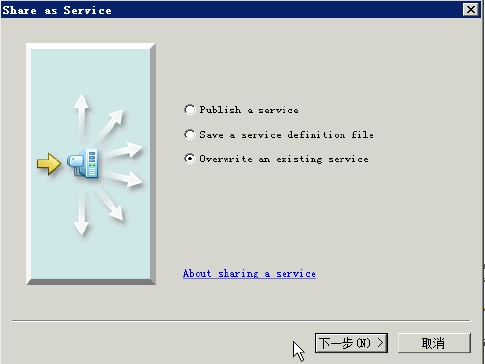
\includegraphics[width=0.7\textwidth]{chp07_GIS数据重新发布步骤1.jpg}
  \caption{GIS数据发布步骤3\label{fig:chp07_GIS数据重新发布步骤1} }
\end{figure}

\item 在弹出的 Overwrite an Existing Service 对话框中, Choose a connection 位置选
择 arcgis on localhost\_6080(admin), service 列表中选中 SZJT, 然后点击下一步按钮(见图\ref{fig:chp07_GIS数据重新发布步骤2});

\begin{figure}[!ht]
  \centering
  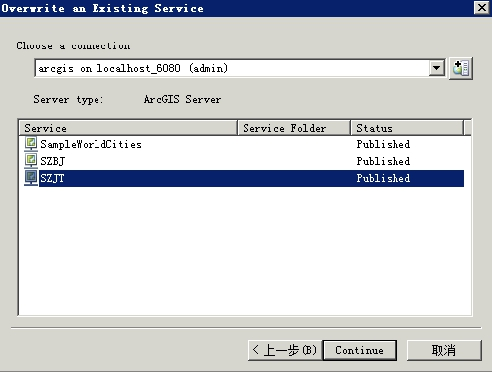
\includegraphics[width=0.7\textwidth]{chp07_GIS数据重新发布步骤2.jpg}
  \caption{GIS数据发布步骤4\label{fig:chp07_GIS数据重新发布步骤2} }
\end{figure}

\item 如图\ref{fig:chp07_GIS数据重新发布步骤1}所示,在弹出的 Service Editor 对话框中, 点击右上角 Analyze 按钮, 分析完成后如果显示“ 0 Errors”则表示没有错误,否则就要排查错误(如果出现 warnings可以忽略);

\begin{figure}[!ht]
  \centering
  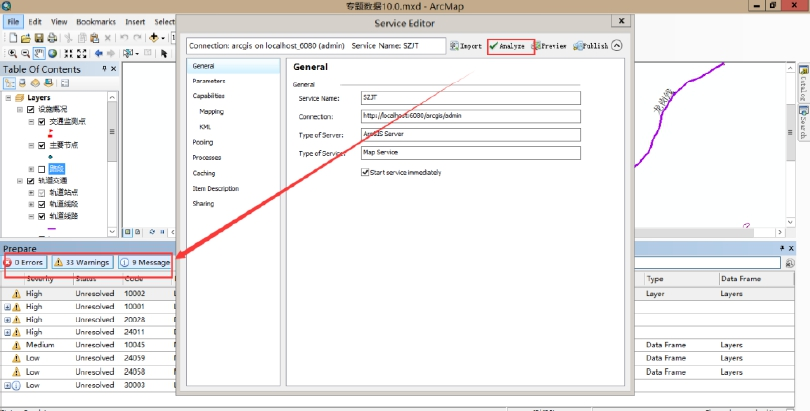
\includegraphics[width=\textwidth]{chp07_GIS数据重新发布步骤3.jpg}
  \caption{GIS数据发布步骤5\label{fig:chp07_GIS数据重新发布步骤3} }
\end{figure}

\item 最后, 点击右上角 Publish 按钮进行地图服务发布, 发布成功后会弹出对话框
提示“ The service has been published sucessfully.”。
\end{nbeae}

\subsection{新版本重新部署}
\pyear 年度更新中只涉及了前端源代码的修改, 因此新版本重新部署工作只
需要对前端服务进行重新部署, 不涉及后台服务。

由于深圳市交通仿真系统( 二期) 已建成查询系统的中间件软件采用的是
weblogic, 所以首先需要将前端代码打成 war 包。 具体的操作步骤如下:

\begin{nbeae}
\item 首先,从 windows 控制台进入到前端代码所在文件夹 szgisviewer;
\item 然后, 执行命令 $jar \ {\text -} cvf \ szgisviewer.war \ *.*$,执行完成后会出现如下窗体, 表
明打包成果,此时在 szgisviewer 文件夹根目录下会产生 szgisviewer.war 文件;

\item 将 szgisviewer.war 文件拷贝一份放入查询系统应用服务器(具体配置见附录\ref{chpt:附录B})
上的weblogic安装目录中: $C:\backslash Middleware\backslash user\_projects\backslash domains\backslash base\_domain\backslash \\ webapps$(如果没有 webapss 文件夹,需要自行新建)。
\end{nbeae}

然后, 按照 weblogic 的服务发布步骤完成系统部署工作, 具体流程如下:

\begin{nbeae}
\item 执行查询系统应用服务器 $C:\backslash Oracle\backslash Middleware\backslash user\_projects\backslash domains\backslash\\ base\_domain$ 文件夹中的 startWebLogic.bat, 
启动 weblogic( weblogic 管理配置见附录\ref{chpt:附录B}), 输入账号密码后进入管理主页面;

\item 在管理主页面上, 依次点击左上角“锁定并编辑”按钮,左边导航栏“部署”
条目,和页面中部“安装”按钮,如图\ref{fig:chp07_新版本重新部署步骤2}所示:

\begin{figure}[!ht]
  \centering
  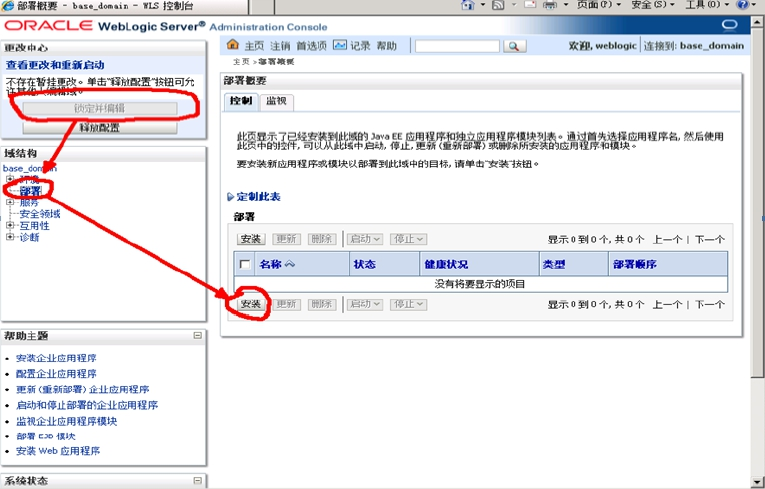
\includegraphics[width=0.8\textwidth]{chp07_新版本重新部署步骤2.jpg}
  \caption{新版本重新部署步骤2\label{fig:chp07_新版本重新部署步骤2} }
\end{figure}

\item 在跳转后的页面下部“当前位置” 中选择“ szgisviewer.war”, 点击下一步按钮;
\item 在跳转后的页面中选择“ 将此部署安装为应用程序” , 点击下一步按钮;
\item 后续两个页面都按默认设置,并点击下一步按钮;
\item 最后,当出现如下页面时,先点击“ 保存” 按钮,然后再点击“激活更改”
(见图\ref{fig:chp07_新版本重新部署步骤6})。

\clearpage

\begin{figure}[!ht]
  \centering
  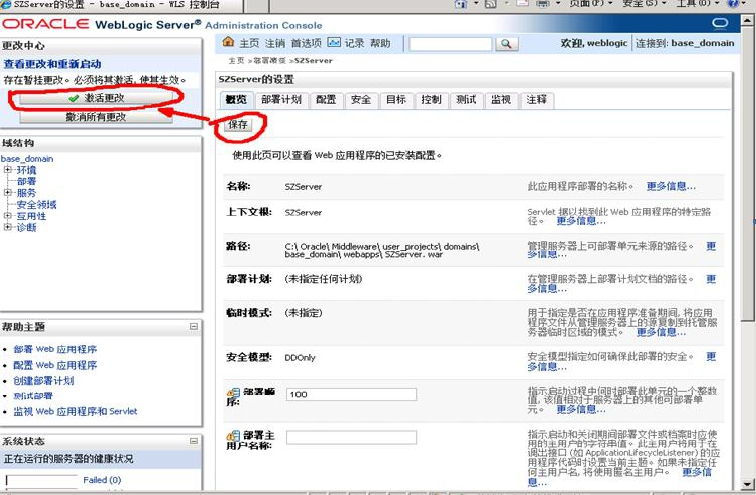
\includegraphics[width=0.8\textwidth]{chp07_新版本重新部署步骤6.jpg}
  \caption{新版本重新部署步骤6\label{fig:chp07_新版本重新部署步骤6} }
\end{figure}
\end{nbeae}

在项目部署完成后, 还需要将 weblogic 服务重新启动, 具体流程如下:

\begin{nbeae}
\item 在 weblogic 管理页面中, 点击锁定并编辑按钮,勾选文件 szgisviewer 和
szserver,然后点击启动->为所有请求提供服务(见图\ref{fig:chp07_服务启动步骤1});

\begin{figure}[!ht]
  \centering
  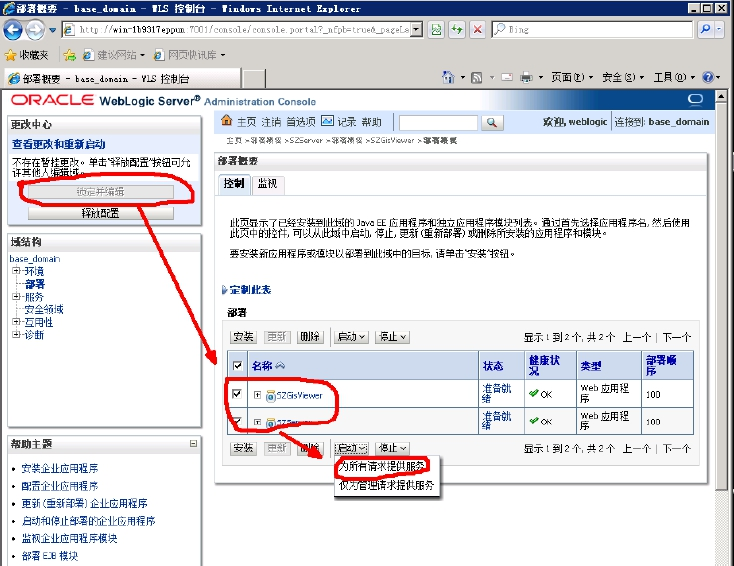
\includegraphics[width=0.8\textwidth]{chp07_服务启动步骤1.jpg}
  \caption{weblogic服务启动步骤1\label{fig:chp07_服务启动步骤1} }
\end{figure}

\item 在跳转后的“启动部署” 页面中,点击“是” 按钮, 启动成功后出现“已经
将启动请求发送到了所选部署”提示(见图\ref{fig:chp07_服务启动步骤2})。

\begin{figure}[!ht]
  \centering
  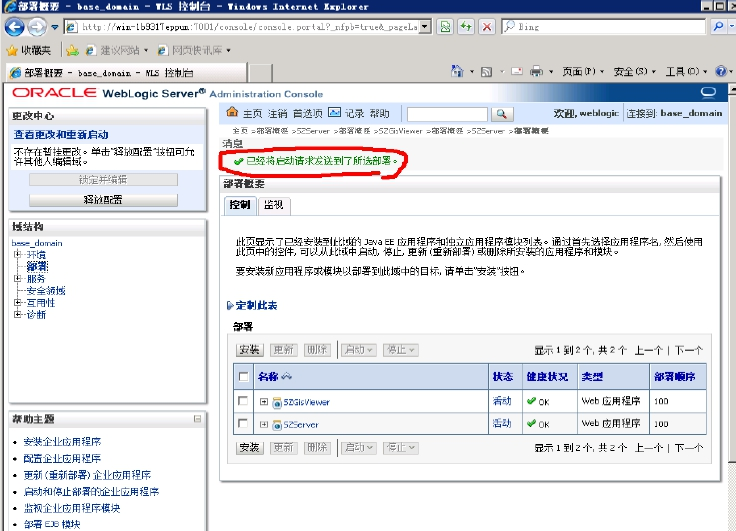
\includegraphics[width=0.8\textwidth]{chp07_服务启动步骤2.jpg}
  \caption{weblogic服务启动步骤2\label{fig:chp07_服务启动步骤2} }
\end{figure}
\end{nbeae}

至此,新版本系统的部署工作全部完成,可以在前端浏览器中查询到最新的
GIS 地图数据和挖掘计算后的各类交通指标数据。

\section{年度更新成果}
数据查询系统是一个面向用户的展示系统,因此年度更新的最终成果是一个
可在浏览器中查看的系统新版本。 按照上述几节的更新工作,最终系统发布的网
址为$http://192.168.114.101:7001/szgisviewer/$, 在全委的内网环境中都可以正常访
问, 登录账户为 admin, 密码为 pass。登录后的主界面见图\ref{fig:chp07_新版本交通信息查询分析系统主界面}。

\begin{figure}[!ht]
  \centering
  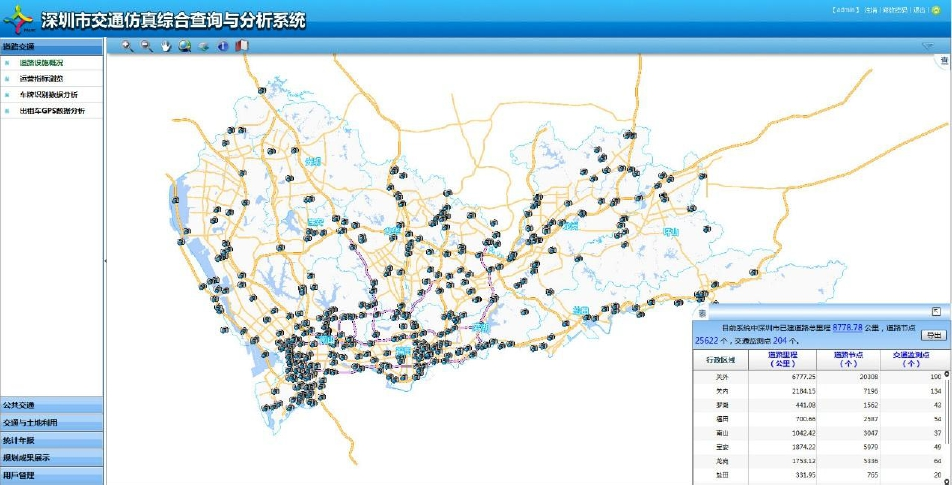
\includegraphics[width=\textwidth]{chp07_新版本交通信息查询分析系统主界面.jpg}
  \caption{新版本交通信息查询分析系统主界面\label{fig:chp07_新版本交通信息查询分析系统主界面} }
\end{figure}

\item 新版本系统内的功能较多,但是大致可以分为以下几类查询功能:

\begin{cit}
\item 总体指标查询
\item 车牌识别数据查询
\item 轨道交通数据查询
\item 常规公交数据查询
\end{cit}

\subsection{总体指标查询}
主要更新内容包括全市、 行政区和道路等级的里程、车速、流量、 饱和度和
高峰小时比等指标, 这些功能包含在“道路设施概况” 和“运营指标浏览” 中。

\begin{figure}[!ht]
  \centering
  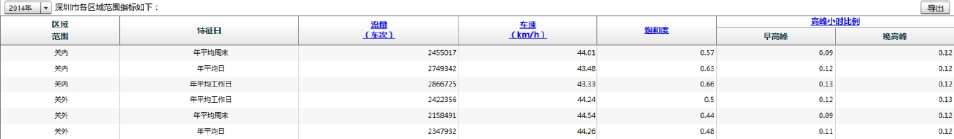
\includegraphics[width=\textwidth]{chp07_总体指标查询.jpg}
  \caption{总体指标查询\label{fig:chp07_总体指标查询} }
\end{figure}

\subsection{车牌识别数据查询}
主要更新内容包括重要路段和交叉口车流量,包括全市 100 多个监测点,分
全天、早晚高峰时段,以及不同时段变化趋势。例如, 图\ref{fig:chp07_2017年梅林关口特征时段车流量查询}是\pyear 年更新后的
梅林关口在特征时段( 早高峰、晚高峰、 全天) 的车流量。

\begin{figure}[!ht]
  \centering
  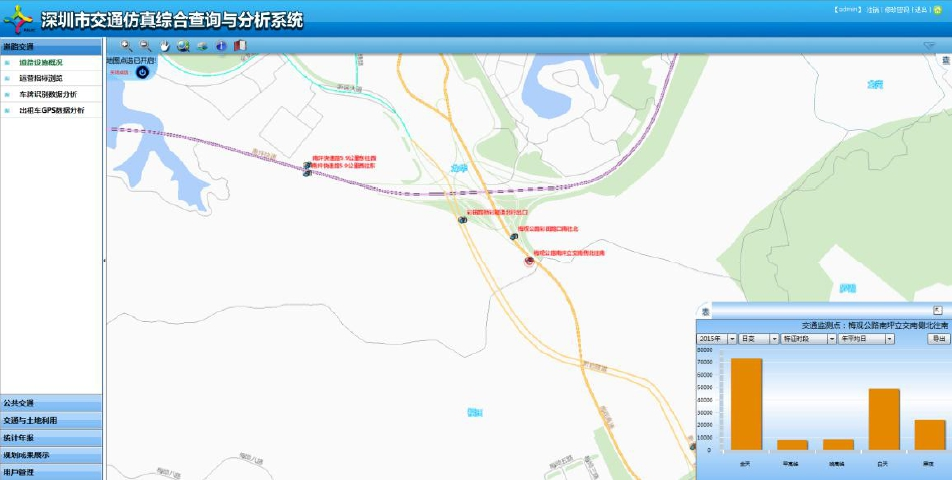
\includegraphics[width=\textwidth]{chp07_2017年梅林关口特征时段车流量查询.jpg}
  \caption{\pyear 年梅林关口特征时段车流量查询\label{fig:chp07_2017年梅林关口特征时段车流量查询} }
\end{figure}


\subsection{轨道交通数据查询}
主要更新内容包括轨道线路和站点客流量查询,分全天、早晚高峰,以及不
同时段变化趋势;轨道换乘流量, 包括不同线路之间的换乘、轨道和巴士换乘以
及换乘站流量,分全天、早晚高峰; 轨道 OD 流量查询,包括不同站点之间和不
同交通小区之间,分全天、早晚高峰; 轨道断面流量查询, 分全天、早晚高峰。

\begin{figure}[!ht]
  \centering
  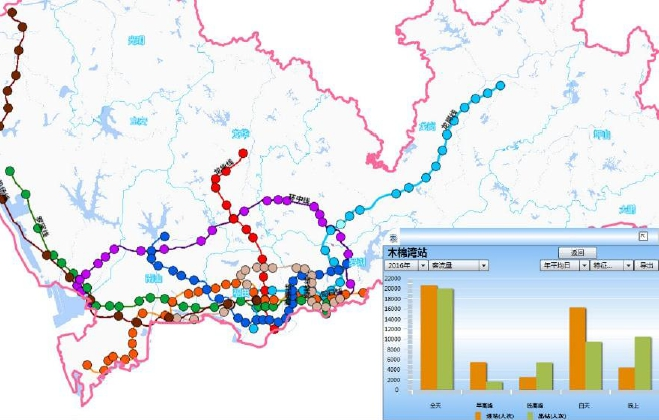
\includegraphics[width=\textwidth]{chp07_2017年轨道线路流量查询.jpg}
  \caption{\pyear 年轨道线路流量查询(三号线)\label{fig:chp07_2017年轨道线路流量查询} }
\end{figure}

\begin{figure}[!ht]
  \centering
  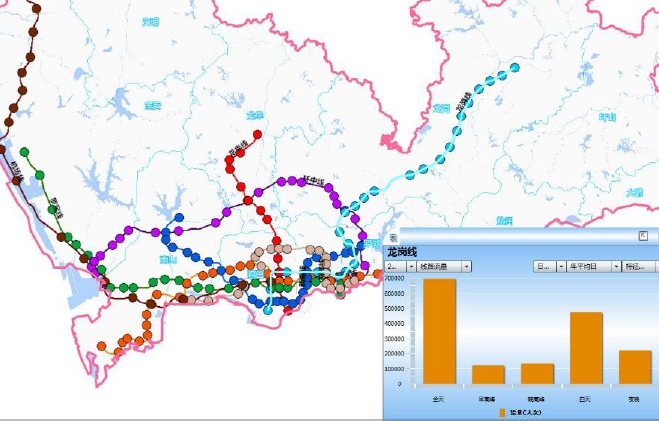
\includegraphics[width=\textwidth]{chp07_2017年轨道站点流量查询.jpg}
  \caption{\pyear 年轨道站点流量查询(木棉湾站)\label{fig:chp07_2017年轨道站点流量查询} }
\end{figure}

\begin{figure}[!ht]
  \centering
  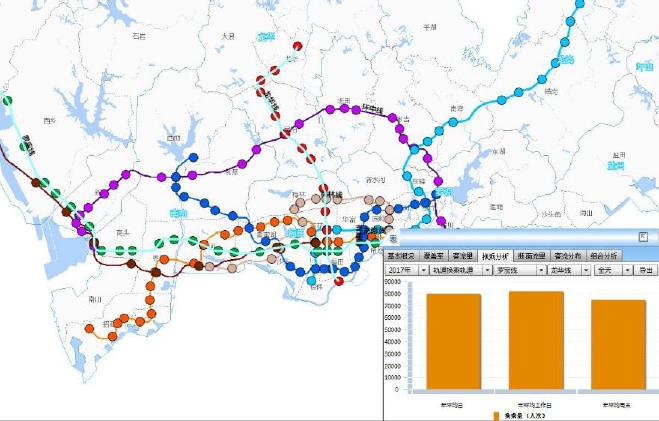
\includegraphics[width=\textwidth]{chp07_2017年轨道换乘流量查询.jpg}
  \caption{\pyear 年轨道换乘流量查询(一号线和四号线)\label{fig:chp07_2017年轨道换乘流量查询} }
\end{figure}

\begin{figure}[!ht]
  \centering
  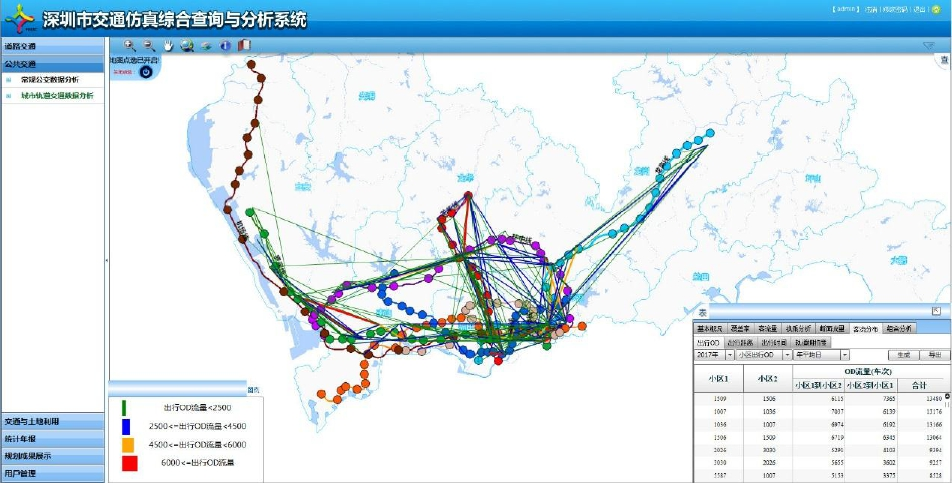
\includegraphics[width=\textwidth]{chp07_2017年轨道站点间OD客流查询.jpg}
  \caption{\pyear 年轨道站点间OD客流查询\label{fig:chp07_2017年轨道站点间OD客流查询} }
\end{figure}

\begin{figure}[!ht]
  \centering
  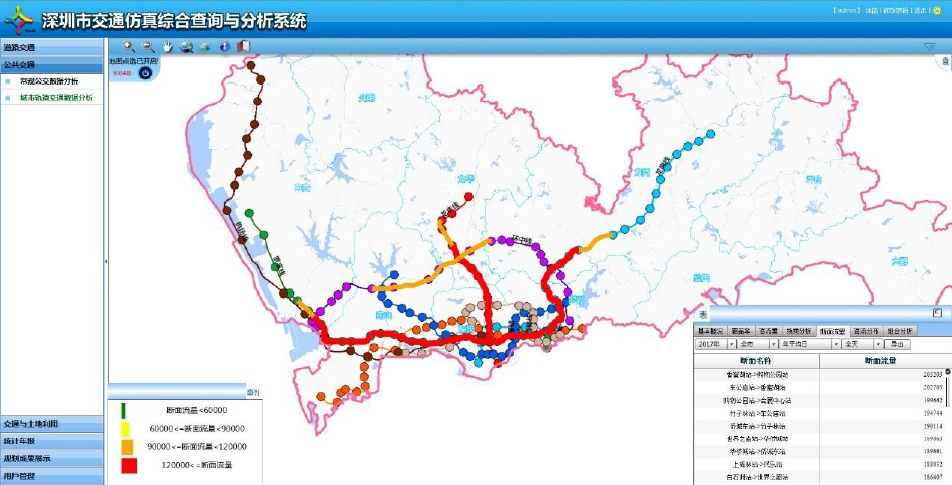
\includegraphics[width=\textwidth]{chp07_2017年轨道断面客流量查询.jpg}
  \caption{\pyear 年轨道断面客流量查询\label{fig:chp07_2017年轨道断面客流量查询} }
\end{figure}

\subsection{常规公交数据查询}
主要更新内容包括常规公交总体客流量查询; 常规公交换乘量查询,包括巴
士换乘巴士和巴士换乘轨道; 常规公交方式出行的 OD 流量和出行时间,包括不
同站点之间和不同交通小区之间。

\begin{figure}[!ht]
  \centering
  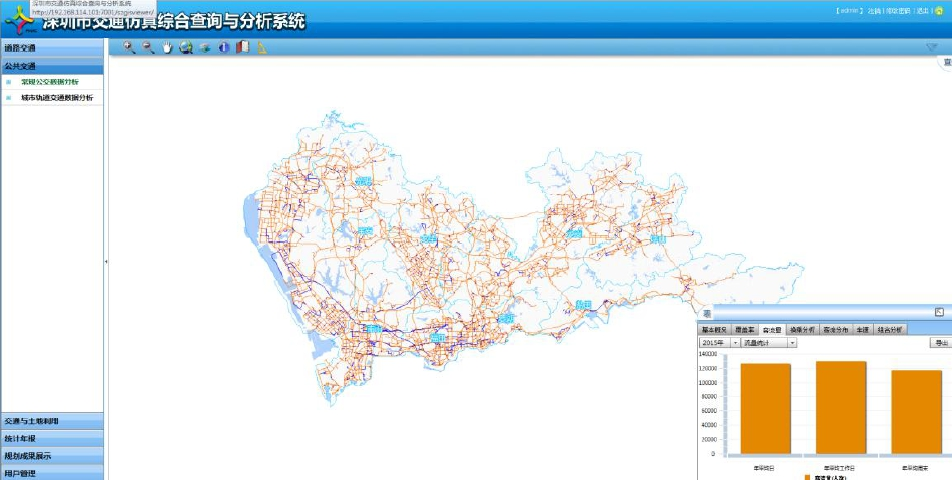
\includegraphics[width=\textwidth]{chp07_2017年常规公交总体客流量查询.jpg}
  \caption{\pyear 年常规公交总体客流量查询\label{fig:chp07_2017年常规公交总体客流量查询} }
\end{figure}

\makeatletter
\setlength{\@fptop}{0pt}
\makeatother
